\documentclass{sig-alternate-05-2015}
\usepackage{amsmath}
\usepackage[T1]{fontenc}
\newcommand\numberthis{\addtocounter{equation}{1}\tag{\theequation}}

\begin{document}

\author{Alun Meredith\vspace{-2ex}% Toggle commenting out the command
}
\title{Options Pricing \vspace{-2ex}% to see the effect
}
\maketitle

\vspace{-30mm}

\begin{abstract}
\end{abstract}

\section{Noise Filtering}
\textbf{Separate the noise from underlying trend through various models}

\subsection{Auto-regressive models}

Auto-regression models the behaviour of stock price today as a function of the previous days plus some random noise:

\begin{equation}
y_{t} = \sum_{i=1}^{Order} \beta_i x_{t-i} + \epsilon_t
\end{equation}

It is natural to think of stock price as auto-regressive; today's price is yesterdays price + returns. Although it is not clear what order the function would take and a stationary form clearly over-simplifies, for example volatility (size of the noise term) is known to not be stationary. There are extensions to this model such as GARCH models which account for varying volatility and ARIMA processes which include moving average effects. 

An auto-regression model can easily by computed by minimising least squares with the pseudo-inverse for a set of time lagged features, such as for Order = 3 below:

\begin{align}
\begin{bmatrix}
  x_1 & x_2 & x_3 \\ 
  x_2 & x_3 & x_4 \\ 
  \vdots & \vdots & \vdots \\ 
  x_{n-3} & x_{n-2} & x_{n-1} \\
\end{bmatrix}
\begin{bmatrix}
  \beta_1 \\ 
  \beta_2 \\ 
  \vdots \\ 
  \beta_{Order} \\ 
\end{bmatrix}
=
\begin{bmatrix}
  y_4 \\ 
  y_5 \\ 
  \vdots \\ 
  y_n \\ 
\end{bmatrix}
\end{align}

\subsection{Kalman Filtering}
Another method of filtering the noise of a signal is using Kalman filtering. This is a state based model with the advantage that it is updated iteratively. This means that upon receiving new data the model isn't recomputed but updated, a much more computationally efficient process. 

The state space model is defined as an underlying value $\theta$ following an order 1 autoregressive function and an observed stock price as $z$ which is the underlying value augmented by some noise. There are only two parameters which need to be defined; the noise of the observation $V$, estimated as the variance variance in residual from the AR model and the noise of the underlying value $W$ which is tuned empirically using cross validation and RMSE. 

\begin{align}
&z_t = \theta_t + v_t \qquad &v_t \sim N(0, V) \\
&\theta_t = \theta_{t-1} + \omega_t \qquad &\omega_t \sim N(0, W) \\
&\theta_0 \sim N(m_0, V)
\end{align}

This leads to the following set of iterative update equations:
\begin{align*}
\mathtt{Prediction} \\
\hat{\theta}_{t|t-1} = \hat{\theta}_{t|t-1} \\
P_{t|t-1} = P_{t-1|t-1} + W \\
\mathtt{Correction} \\
r_t = z_t - \hat{\theta}_{t|t-1} \\
S_t = P_{t|t-1} + V \\
K_t = P_{t|t-1}S_t^{-1} \\
\hat{\theta}_{t|t} = \hat{\theta}_{t|t-1} + K_tr_t \\
P_{t|t} = (1 - K_tH_t)P_{t|t-1}
\end{align*}

We simulate an autoregressive function to test the Kalman filtering: 

\begin{equation}
 Y = 0.7Y_{t-1} + 0.3Y_{t-2} + \eta \qquad \eta \sim N(0,0.1) \label{simulation}
\end{equation}

Figures \ref{fig:W_variation} and \ref{fig:Weight_Estimation} describes the effect of Kalman smoothing. Figure \ref{fig:Weight_Estimation} shows how the Kalman filtering algorithm estimates the underlying weights of the autoregressive model. It shows that there is high variance initially but quickly gets close to the correct weights but doesn't converge to them. Figure \ref{fig:W_variation} shows the effect of the size of the evolution noise $W$. As the value decreases smoothing increases, this is due to a higher level of certainty $P$ for the current prediction and therefore less weight associated to the correction. 

\begin{figure}[ht]
	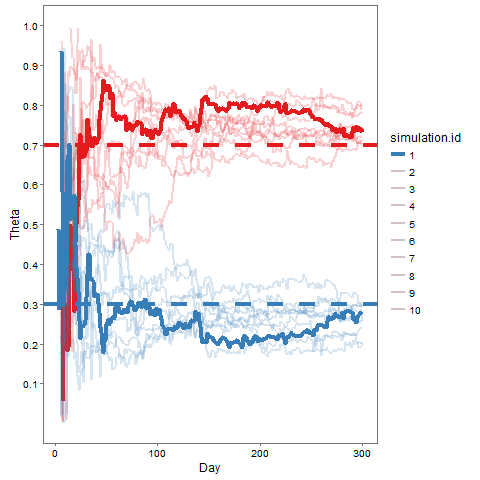
\includegraphics[width=\linewidth]{Test_Weight_Estimation.png}
	\centering
	\caption{The prediction of underlying auto-regression weights from Kalman filtering over time for simulated data \eqref{simulation} (W = 1e-4)}
			\label{fig:Weight_Estimation}
\end{figure}

\begin{figure}[ht]
	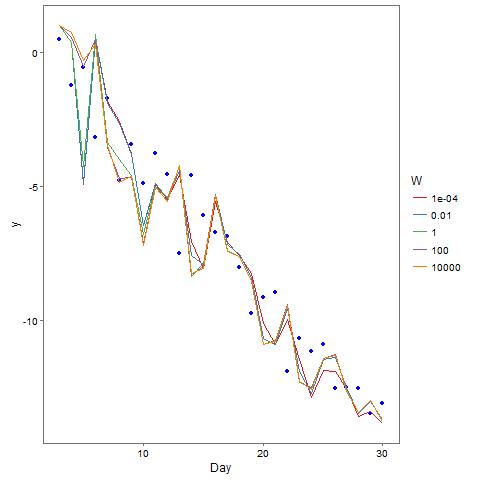
\includegraphics[width=\linewidth]{W_variation.png}
	\centering
	\caption{The Kalman smoothing vs. observed values for a variety of W values for simulated data \eqref{simulation}}
			\label{fig:W_variation}
\end{figure}

Evaluating a the Kalman Smoothing and AR models for a variety of orders and W values we can find the optimal values for these parameters. Figure \ref{fig:RMSE_real} shows that low values of W and order or high values of both W and order are best. This makes some sense as low W retains previous predictions more, if the underlying model was a high order autoregressive function then low order Kalman filtering could 'get access to' the higher order data by having low W. If the Kalman filtering is high enough order it can 'forget' about the earlier data by having high W. Order 1 systems effectively predict tomorrow's value equals today's value because no intercept was used in our model. Finally Kalman filtering never reaches the accuracy of RMSE but this is in some sense not fair as the AR model has seen all the data and is fitting to a training set whereas the Kalman smoothing is predicting on unknown data at each step. A more accurate assessment of RMSE for AR could be done by computing the AR model iteratively for each t up to t-1 and then predicting the next value with it. 

\begin{figure}[ht]
	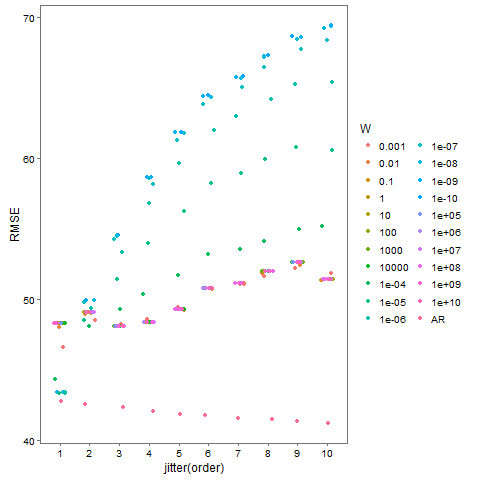
\includegraphics[width=\linewidth]{RMSE_order_real.png}
	\centering
	\caption{RMSE of Kalman smoothing and AutoRegression against Historic Data for a variety of orders and W values, x value is "jittered" to show overlapping points clearly}
			\label{fig:RMSE_real}
\end{figure}

Finally we can see the effects of the 3 best models (Kalman with low order and W, high order and high W and Auto-regression) in figure \ref{fig:DifferentModels}. It shows low order/W kalman being very similar to the auto-regression model while high W/order Kalman while similar doesn't smooth as much.  

\begin{figure}[ht]
	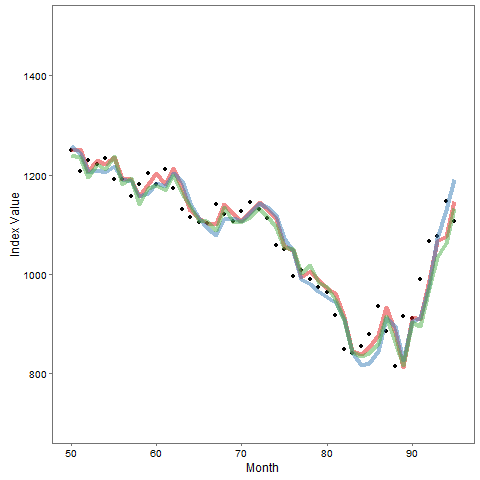
\includegraphics[width=\linewidth]{DifferentModels.png}
	\centering
	\caption{Effects of smoothing for: \textbf{Kalman} Order 1, W 1e-7 (red), \textbf{Kalman} Order 5, W 1e5 (blue) and \textbf{Autoregression}, Order 3 (green). On a subset of the data (Months 50-100, chosen to give Kalman filters enough time to train and capture shifts in the direction of the data)}
			\label{fig:DifferentModels}
\end{figure}

\section{Lasso Regularisation}
 
\clearpage 
\bibliographystyle{abbrv}
\bibliography{sigproc}  % sigproc.bib is the name of the 



\end{document}